\section{TODO: Quadratic Form}
    \begin{Def}\label{def-quadratic}
        A \textbf{quadratic form on $\Rn$} is a function $Q: \Rn\to \mathbb{R}$ whose input vector $\B{x}$ can be computed by an expression of the form:.
        \begin{equation*}
            Q(\B{x}) = \B{x}^{\top}A\B{x}
        \end{equation*}
        where $A$ is a $n\times n$ \textit{symmetric matrix} and called \textbf{the matrix of the quadratic form}. Since $A$ is symmetric, $Q(\B{x})$ can also be expressed as:
        \begin{equation*}
            Q(\B{x}) = \B{x}^{\top}A\B{x} = \sum_{i = 1}^n a_{ii}x_i^2 + 2\sum_{i = 1}^{n - 1}\sum_{j = i + 1}^n a_{ij}x_{i}x_{j}
        \end{equation*}
    \end{Def}
    \subsection{Change of Variable in a Quadratic Form}
    Let $\B{x}\in\Rn$, then a \textit{change of variable} is an equation of the form
    \begin{equation*}
        \B{x} = P\B{y},\quad \text{or equivalently} \quad \B{y} = P^{-1}\B{x}
    \end{equation*}
    where $P$ is a non-singular $n\times n$ matrix. It is easy to see $\B{y} = \coo{x}{B}$, where $\mathcal{B}$ is the set of columns of $P$. Then
    \begin{equation}
        Q(\B{x}) = \B{x}^{\top}A\B{x} = (P\mathbf{y})^{\top} A(P\B{y}) = \B{y}^{\top}(P^{\top}AP)\B{y} = \T{\B{y}}D\B{y}
    \end{equation}
    which uses the fact that $A$ is symmetric.
    \begin{Ex}
        Let
        \begin{equation*}
            A = \begin{bmatrix}
                a & c\\
                c & b
            \end{bmatrix}, \B{x} = \begin{bmatrix}
                x_1\\
                x_2
            \end{bmatrix}
        \end{equation*}
        where $A$ has eigenvalues $\lambda_1$ and $\lambda_2$. Then
        \begin{equation*}
            Q(\B{x}) = \T{\B{x}}A\B{x} = a^2x_1^2 + b^2x_2 + 2cx_1x_2
        \end{equation*}
        By making the change of variable:
        \begin{equation}\label{change-of-variable}
            Q(\B{x}) = Q'(\B{y}) = \T{\B{y}}D\B{y} =  \lambda_1^2y_1^2 + \lambda_2^2y_2^2
        \end{equation}
        \begin{Rem}
            If we let $Q'(\B{y}) = 1$, then $\lambda_1^2y_1^2 + \lambda_2^2y_2^2 = 1$ represents \textbf{\textcolor{red} {an ellipse centred at the origin}}.
        \end{Rem}
    \end{Ex}
    \begin{Thm}
        \textbf{The Principal Axes Theorem}:
        Let $A\in\Rnn$ be a symmetric matrix. Then there is an orthogonal change of variable, $\B{x} = P\B{y}$, that transforms the quadratic form $\quadratic{x}{A}$ into a quadratic form $\quadratic{y}{D}$ with no cross-product term. The columns of $P$ are called the \textbf{principal axes} and $\B{y}$ is the coordinate of $\B{x}$ relative to the columns of $P$.
    \end{Thm}
    \subsection{A Geometric View of Principal Axes}
    Suppose $Q(\B{x}) = \quadratic{x}{A} = k$, where $A$ is $2\times 2$ symmetric matrix and $k\in\mathbb{R}$.
    The set of all $\B{x}\in\mathbb{R}^2$ that satisfy
    \begin{equation*}
        \quadratic{x}{A} = \quadratic{x}{A} = k
    \end{equation*}
    It can be expressed as
    \begin{equation*}
        a^2x_1^2 + bx_1x_2 + c^2x_2^2 + dx_1 + ex_2 + f = 0
    \end{equation*}
    which either corresponds to 
    \begin{enumerate}
        \item an ellipse (or a circle):
        \begin{equation}\label{ellipse}
            a^2x_1^2 + bx_1x_2 + c^2x_2^2 + dx_1 + ex_2 + f = 0,\ ac> 0
        \end{equation}
        \item a hyperbola:
        \begin{equation}\label{hyperbola}
            a^2x_1^2 + bx_1x_2 + c^2x_2^2 + dx_1 + ex_2 + f = 0,\ ac < 0
        \end{equation}
        \item two intersecting lines, if the \cref{ellipse} can be factorized to
        \begin{equation*}
            (\alpha_1x_1 + \beta_1x_2 + \gamma_1)(\alpha_2x_1 + \beta_2x_2 + \gamma_2) = 0
        \end{equation*}
        \item a single point:
        \begin{equation*}
            (x_1 - x_0)(x_2 - y_0) = 0
        \end{equation*}
    \end{enumerate}
    If $A$ is a diagonal matrix, the graph is in \textit{standard position}, which implies that the ellipse or the hyperbola is centred at the origin. Therefore, the \cref{ellipse} can be written as:
    \begin{equation*}
        \cfrac{x_1}{a^2} + \cfrac{x_2}{b^2} = 1,\ a>0,\ b > 0
    \end{equation*}
    The \cref{hyperbola} can be written as:
    \begin{equation*}
        \cfrac{x_1}{a^2} - \cfrac{x_2}{b^2} = 1,\ a>0,\ b > 0
    \end{equation*}
    \textbf{\textcolor{cyan}{Find the \textit{principal axes} (determined by the eigenvectors of $A$) amounts to finding a new coordinate system with respect to which the graph is in standard position (centred at the origin)}}, as shown below:
    \begin{figure}[ht]
    \centering
    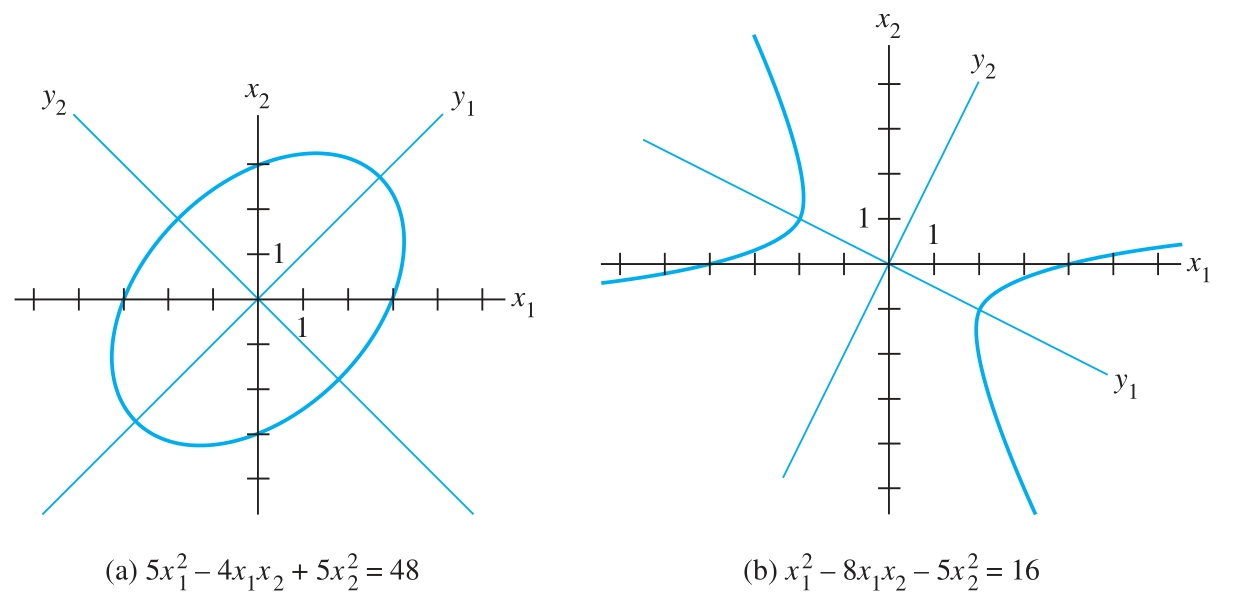
\includegraphics[width=0.75\textwidth]{images/principal-axes.png}
    \caption{Finding the principal axes.}
   %\label{Find the principal axes.}
    \end{figure}
    
    \subsection{Classifying Quadratic Forms}
    \begin{Def}\label{quad-def}
        A quadratic from $Q$ is
        \begin{enumerate}[(a)]
            \item \textbf{positive definite} if $\forall \B{x} \neq \B{0}:Q(\B{x}) > 0$
             \item \textbf{negative definite} if $\forall \B{x} \neq \B{0}:Q(\B{x}) < 0$
             \item \textbf{indefinite} if $Q(\B{x})$ assumes both positive and negative values.
             \item \textbf{positive semi-definite} if $\forall \B{x}:Q(\B{x}) > 0$
             \item \textbf{negative semi-definite} if $\forall \B{x}:Q(\B{x}) < 0$
        \end{enumerate}

    \end{Def}
        As shown in the figure 2.
        \begin{figure}
        \centering
        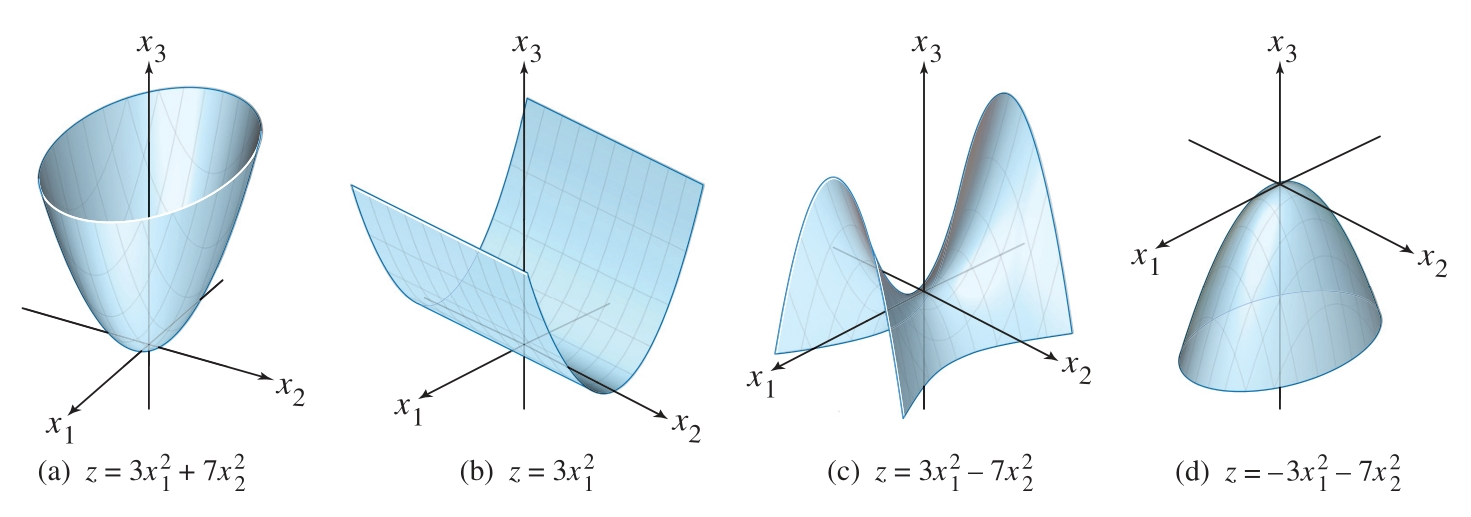
\includegraphics[width=0.75\textwidth]{images/quadratic-class.png}
        \caption{Graphs of quadratic forms.}
       %\label{Find the principal axes.}
        \end{figure}
        
    \begin{Thm}\label{11-2}
        \textbf{Quadratic Forms and Eigenvalues}:
        Given a quadratic form $Q(\B{x}) = \quadratic{x}{A}$, then $Q$ is
        \begin{enumerate}[a.]
            \item positive definite if and only if the eigenvalues of $A$ are all positive,
            \item negative definite if and only if the eigenvalues of $A$ are all negative, or
            \item indefinite if and only $A$ has both positive and negative eigenvalues.
        \end{enumerate}
        \begin{proof}
            By the \cref{change-of-variable},
            \begin{equation}
                Q(\B{x}) = \quadratic{x}{A} = \quadratic{y}{D} = \sum_{i = 1}^n  \lambda_iy_i^2
            \end{equation}
            Since $P$ is non-singular, there is a one-to-one relation between $\B{x}$ and $\B{y}$. For any nonzero $\B{x}$, the right side of the equation above coincides with $Q(\B{x})$ for $\B{x}\neq \B{0}$. Thereore, $Q(\B{x})$ is obviously controlled by the signs of the eigenvalues of $A$, in the three ways described in the theorem.
        \end{proof}
        \begin{Rem}
            If $A$ has a nonzero eigenvalue, say $\lambda_k = 0$, then $A\B{x} = 0$ has a non-trivial solution, implying $\exists\B{x}\neq \B{0}: Q(\mathbf{x}) = 0$.
        \end{Rem}
    \end{Thm}